\documentclass[a4paper, 11pt]{article}
\usepackage[francais]{babel}
\usepackage[utf8]{inputenc}
\usepackage[T1]{fontenc}
\usepackage{datetime}
\usepackage{float}
\usepackage{eurosym}
\usepackage{comment} % enables the use of multi-line comments (\ifx \fi)
\usepackage{graphicx}

\usepackage{fullpage} % changes the margin

\begin{document}
%Header-Make sure you update this information!!!!
\noindent
\large\textbf{Groupe Saur - compte-rendu} \hfill \textbf{Distribution de l'eau en Haïti} \\
\normalsize Deknop Céline \hfill Université Catholique de Louvain \\
Hallet Adrien \hfill \today \\
Strebelle Sébastien

\section*{Abstract}
Compte-rendu de la visite du CPO de Saur, à Serris (France) le 21 août 2018
\hrule

\section*{Déroulement}
Accueillis par le directeur d'exploitation, Cyrille Teysonnières, nous avons pu interagir avec ce dernier pendant une entrevue d'1h30. Nous avons commencé par une explication de la démarche, du mémoire et de ses enjeux.
Ensuite, le directeur d'exploitation a dressé un bilan sommaire de la distribution d'eau en général. Enfin, nous avons pu échanger lors d'une séance de questions-réponses autour des thèmes de la distribution d'eau.

\section*{Le Centre de Pilotage Opérationnel}
\begin{figure}[H]
    \centering
    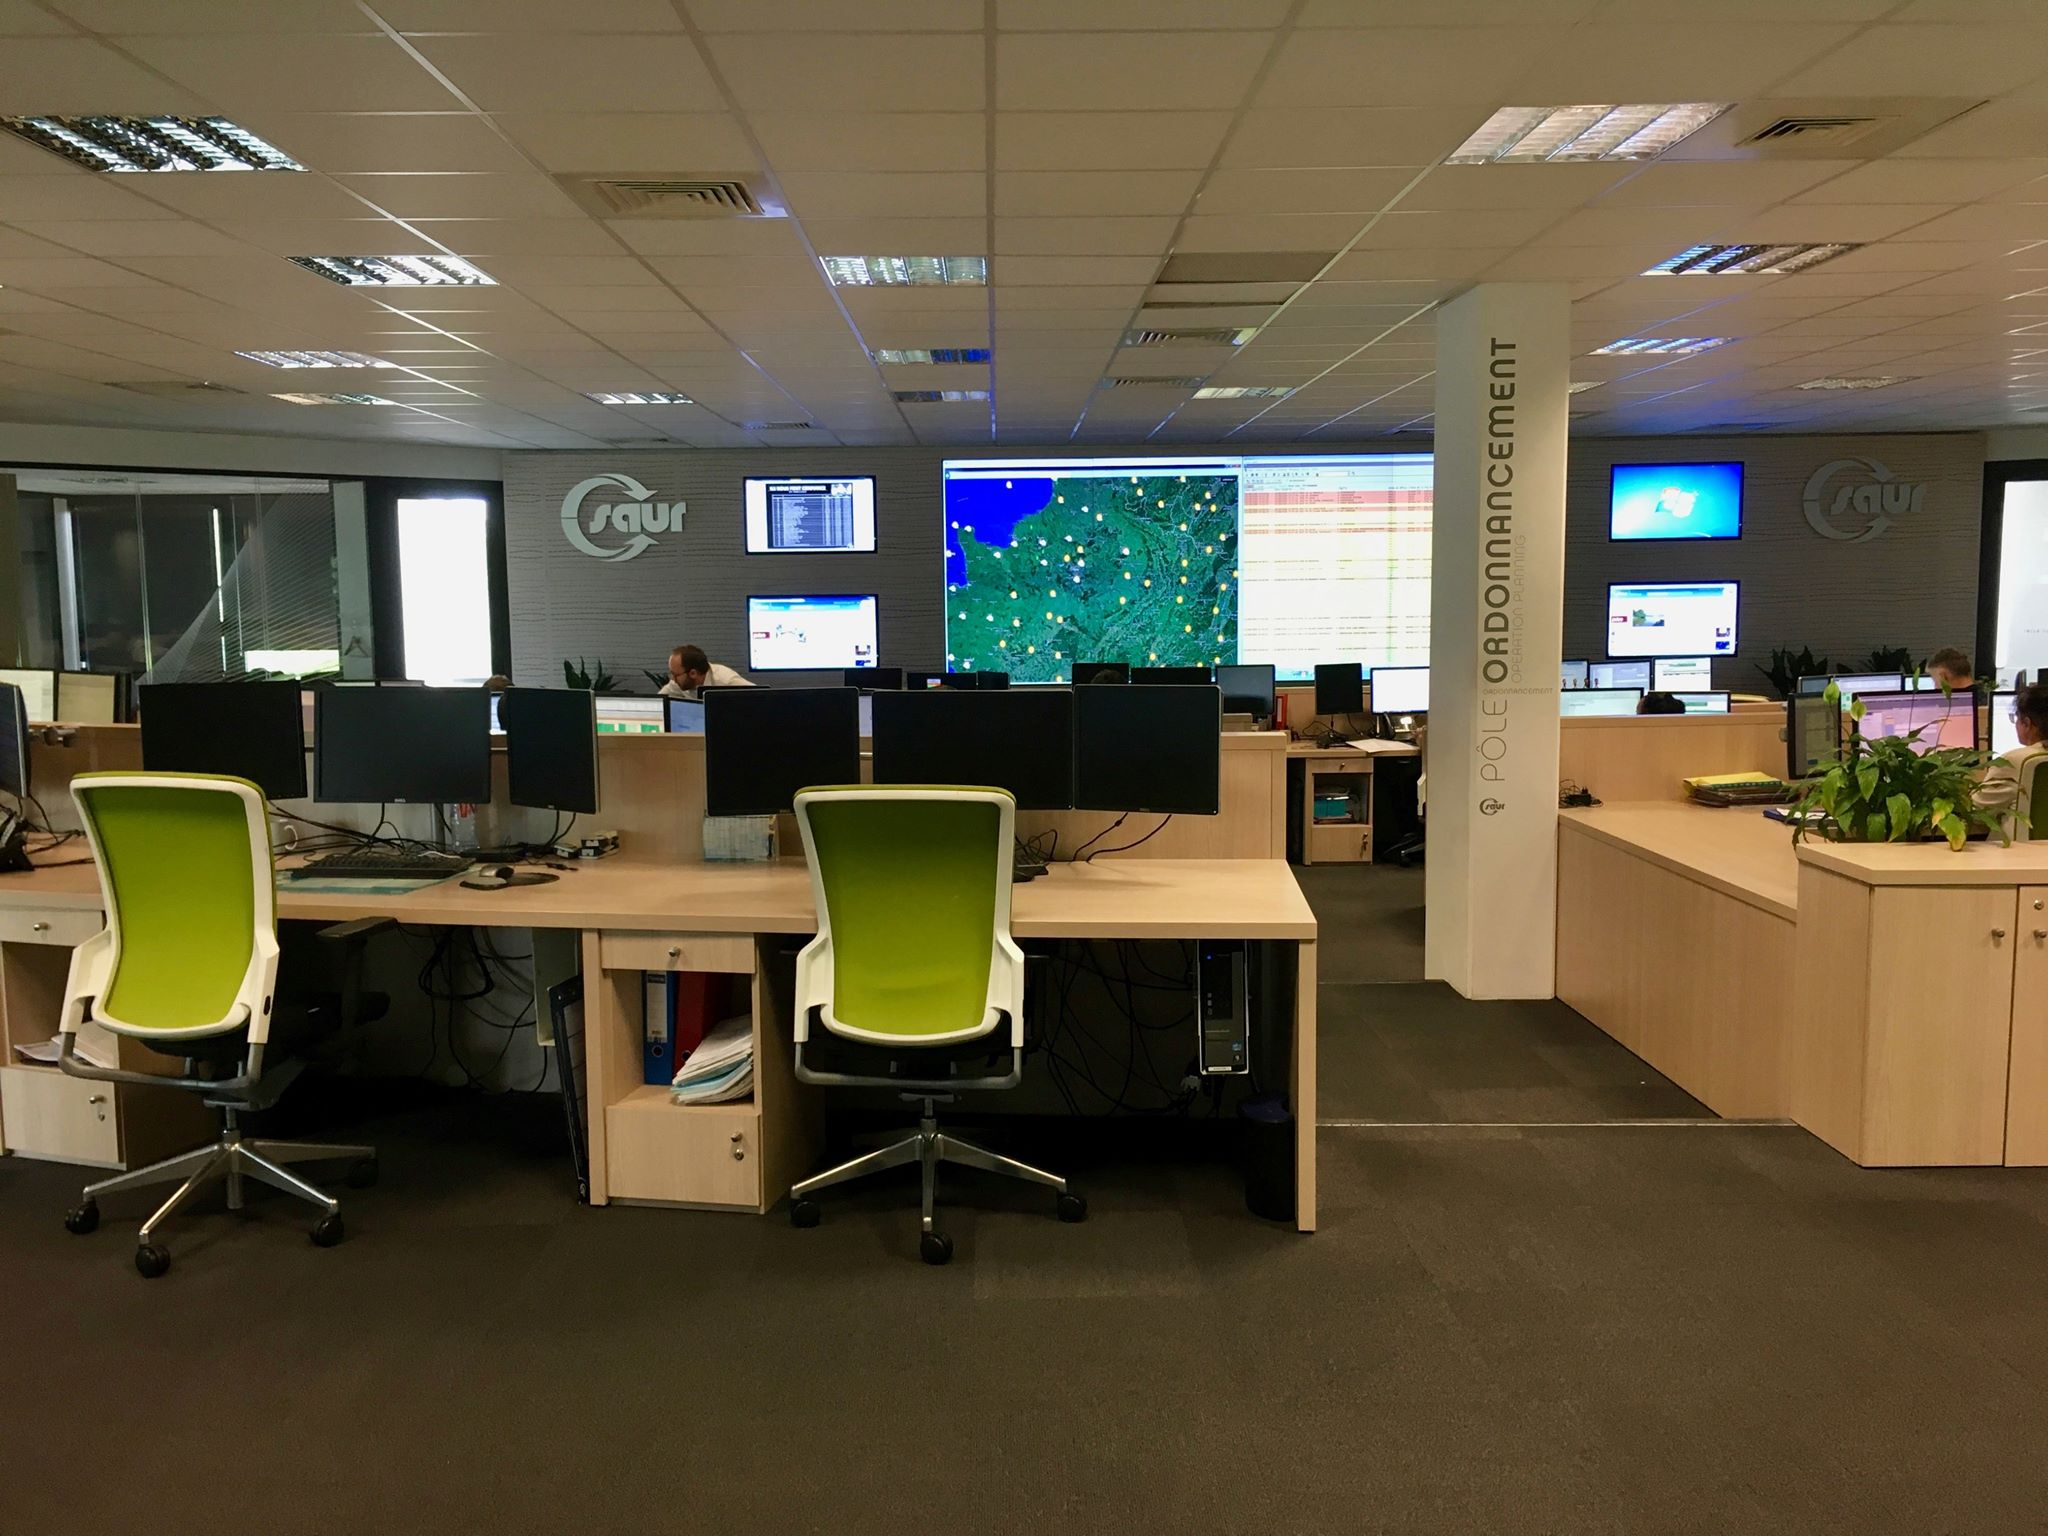
\includegraphics[width=0.8\textwidth]{Entretien_Groupe_Saur/saur}
    \caption{Vue de la salle principale des ordonnanceurs}
    \label{visuel}
\end{figure}
Abrégé \textbf{CPO}, le Centre de Pilotage Opérationnel de Serris dirige les activités du groupe Saur pour la région Île-de-France. Entièrement bureautique, le centre ne comporte aucune installation hydraulique. Les employés présents dans le centre communiquent avec le réseau de manière entièrement informatisée. Ils ont le titre d'\textit{ordonnanceurs} et ils dirigent de dix à trente employés sur le terrain à partir de leur station de travail. On peut scinder leur activité en deux temps forts :
\begin{description}
    \item[Analyse de données] \hfill \\
         L'ordonnanceur reçoit une grande quantité d'information par le biais de tous les capteurs du réseau, il doit être en mesure de les comprendre et de les interpréter (e.g.: fuites).
    \item[Décision et planification] \hfill \\
        Chaque problème découvert donne suite à une résolution ou une mise en attente. C'est à l'ordonnanceur que revient la décision et le type d'opération mis en place. Chaque opération est planifiée et envoyée à un membre de l'équipe, lequel est en contact avec son ordonnanceur.
\end{description}

C'est pourquoi ce lieu est un centre de \textbf{pilotage opérationnel}, car c'est à partir de ces bureaux que toutes les opérations sont pilotées (chaque employé dispose d'une localisation GPS et d'un temps alloué limité pour les opérations). Il est à noter que les ordonnanceurs sont des ingénieurs et ont des formations les rendant généralement capables de comprendre les données rapportées par le programme.



\section*{Système Informatique}
Reflétant l'activité du centre, le système informatique dispose d'outils d'information reflétant l'état du réseau ainsi que d'outils de gestion pour la planification (qui ne nous intéresse pas dans ce contexte).

Le centre utilise \textbf{EPANET}\footnote{Plus d'informations sur EPANET sont disponibles dans l'étude comparative 1} comme logiciel principal. Logiciel gratuit développé par le gouvernement des USA, il est à la base de nombreuses solutions (payantes y compris) informatiques dans le domaine de l'hydraulique.

Nous avons pu constater que le type de système informatique employé ne diffère pas du modèle classique des systèmes ERP. L'eau y est traitée de manière identique aux ressources classiques (employés, horaires, facturation), voire même avec moins d'importance car l'emphase du centre semble réellement centrée sur la productivité des employés à tout prix, l'eau n'étant qu'un produit à vendre.

On constate que le centre fonctionne de manière verticale avec des secteurs bien définis gérés par une hiérarchie établie. Comme dans toute entreprise de ce type, on distingue les équipes de maintenance, développement, facturation, relations humaines, ...

La figure~\ref{visuel} résume les objectifs de notre application. L'écran géant de la pièce, scindé en deux parties, rapporte une information visuelle sur l'état du réseau ainsi qu'un ensemble de données dans le tableur de la partie droite.

\section*{Le réseau de distribution}

Nous cherchions à savoir si le réseau doit être modifié ou adapté pour l'installation d'un système informatisé. En réalité notre interlocuteur nous a appris qu'à une telle échelle il n'y a pas réellement de directives suivies dans le placement du réseau mais surtout une exploitation du réseau existant. Chaque situation est différente et est exploitée au mieux en fonction des besoins.

Par exemple, la connectivité du réseau est principalement un facteur historique ; si certaines zones sont très connectées et la perte d'une conduite a un impact mineur, d'autres sont plus vulnérables de par leur isolation du réseau global. Les coûts d'installation du système n'aidant pas, il est rare d'optimiser le réseau au niveau matériel.

Le directeur du centre insiste beaucoup sur la nécessité de maintenance du réseau tant au point de vue sanitaire (infiltration) qu'économique (fuites).

\section*{Conclusions}

Cette visite nous conforte dans notre idée de réalisation d'un système ERP personnalisé et simplifié afin qu'il soit accesible au destinataire de l'application. La rencontre nous a démontré que l'eau n'était pas un produit traité différemment de toute autre marchandise. Il n'y a pas de mesures spéciales prises dans sa distribution et vente (excepté traitement bio-chimique).

Nous avons vu que l'histoire détermine le réseau de distribution mis en place, puis que le système informatique se greffe par dessus. Le plus important pour le système est donc la collecte des données. La suite des opérations (optimisations, facturation, pompage, maintenance, ...) s'effectue sur la base des ressources existantes.

\end{document}
